\documentclass[resume]{subfiles}


\begin{document}
\begin{multicols}{3}
\section{Circuits}
\subsection{single-supply, inverting, avec référence}
\begin{center}
\includegraphics[scale=1,page=15]{../KiCad/resume-crop.pdf}
\end{center}
$$\boxed{U_{out}=-\frac{R_2}{R_1}\left(U_{in}-U_{ref}\right)+U_{ref}}$$
\subsection{single-supply, non-inverting, sans référence}
\begin{center}
\includegraphics[scale=1,page=16]{../KiCad/resume-crop.pdf}
\end{center}
$$\boxed{U_{out}=\left(1+\frac{R_2}{R_1}\right)\left(U_{in}+U_{ref}\right)+U_{ref}}$$
\columnbreak
\subsection{Single supply, differential, avec référence}
\label{sec_ss_diff_ref}
\begin{center}
\includegraphics[scale=1,page=5]{../KiCad/resume-crop.pdf}
\end{center}
$$\boxed{U_{out}=\frac{R_2}{R_1}\left(U_{in}-U_{in_{inv}}\right)+U_{ref}}$$
\subsection{Single supply, non inverting, unity gain, avec référence}
\begin{center}
\includegraphics[scale=1,page=3]{../KiCad/resume-crop.pdf}
\end{center}
$$\boxed{U_{out}=\left(U_{in}-U_{ref}\right)+\frac{R_1+R_2}{R_2}U_{ref}}$$
Ou, équivalent :
$$\boxed{U_{out}=\frac{U_{in}R_2+U_{ref}R_1}{R_2}}$$
\subsection{Single supply, inverseur, avec référence}
\begin{center}
\includegraphics[scale=1,page=4]{../KiCad/resume-crop.pdf}
\end{center}
$$\boxed{U_{out}=\frac{U_{ref}R_1-U_{in}R_2}{R_1}}$$

\subsection{Single supply, différentiel vers différentiel}
\begin{center}
\includegraphics[scale=1,page=17]{../KiCad/resume-crop.pdf}
\end{center}
Tension de sortie (mesurée entre les deux sortie)
$$\boxed{U_{out}=\left(1+\frac{2R_1}{R_{\text{gain}}}\right)\left(U_{+}-U_{-}\right)}$$
Tension moyenne de sortie (traitillé  bleu)
$$\boxed{U_{\text{mean}}=\frac{U_{+}+U_{-}}{2}}$$
On peut également placer $U_{ref}$ sur $U_{-}$ pour avoir un amplificateur single-ended vers différentiel (à noter que la valeur moyenne de la sortie va varier avec $U_{+}$).\\
On peut le coupler avec \ref{sec_ss_diff_ref} pour avoir une sortie single-ended (tout en gardant une haute impédance d'entrée).
\subsection{Single supply, single-ended vers différentiel}
\begin{center}
\includegraphics[scale=1,page=18]{../KiCad/resume-crop.pdf}
\end{center}
$$\boxed{U_{out}=2\frac{R_2}{R_1}U_{in}}$$
La tension moyenne de sortie (traitillé bleu) est fixée sur $U_{ref}$
$$\boxed{U_{\text{mean}}=U_{ref}}$$
\subsection{Source de courant constante}
\begin{center}
\includegraphics[scale=1,page=25]{../KiCad/resume-crop.pdf}
\end{center}
$$\boxed{I_{out}=\frac{U_{ref}}{R_2}}$$
La résistance $R_1$ n'as pas d'impact sur la sortie
\columnbreak
\section{Autres}
\subsection{Statistiques}
\begin{figure}[H]
\centering
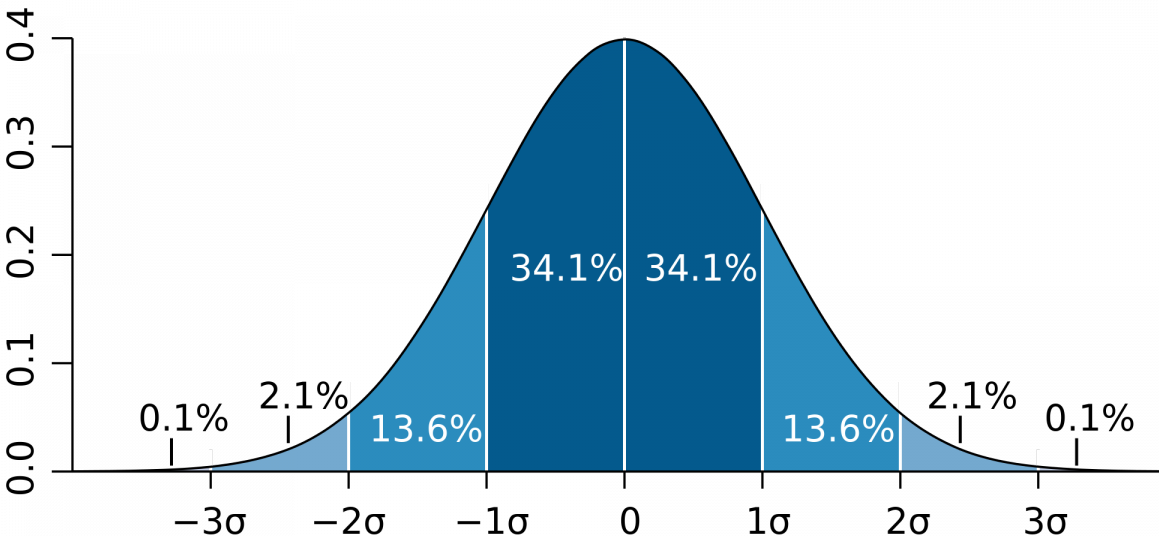
\includegraphics[width=0.6\columnwidth]{gauss.png}
\end{figure}
\subsubsection{Bruit}
Si un bruit est \textbf{aléatoire} (gaussienne), on peut estimer que le \SI{99.9}{\percent} est compris entre $\pm 3.3\sigma$, il est donc possible de passer de pic-pic à rms en multipliant par $2\cdot 3.3$. La valeur rms est $1\sigma$
$$U_{\text{noise}_{pk-pk}}=6.6 U_{\text{noise}_{rms}}$$
\columnbreak
\subsection{Formules}
Inductance
$$LI=UT$$
Charge
$$CU=Q$$
Charge et courant
$$Q=I\Delta T$$
$$\frac{dQ}{dt}=i\longleftrightarrow sQ=i$$
$$i=C\frac{du}{dt}\longleftrightarrow i=sCu$$
$$u=L\frac{di}{dt}\longleftrightarrow u=sLi$$





\end{multicols}
\end{document}